\documentclass{beamer} 

\mode<presentation> {
    \usetheme{ARAMIS}
}

\usepackage[english]{babel}
\usepackage[utf8]{inputenc}

\usepackage{ragged2e}
\usepackage{amsmath,amsthm, amssymb, latexsym}
\usefonttheme[onlymath]{serif}
\boldmath


%%%%%%%%%%%%%%%%
%%% LISTINGS %%%
%%%%%%%%%%%%%%%%
\usepackage{listings}
\definecolor{colString}{rgb}{0.6,0.1,0.1} 
\definecolor{Green}{rgb}{0.1,0.5,0.1}
\lstset{%configuration de listings 
	float=hbp,% 
	language={C},%
	morekeywords={assert, then},%
	basicstyle=\ttfamily\protect\fontsize{26pt}{26pt}\protect\selectfont, % 
	backgroundcolor=\color{white},%
	identifierstyle=\color{black}, % 
	keywordstyle=\color{blue}, % 
	stringstyle=\color{colString}, % 
	commentstyle=\color{Green}, % 
	columns=flexible, % 
	keepspaces=true,  % keeps spaces in text, useful for keeping indentation of code
	escapeinside={\%*}{*)},%
	tabsize=4, % 
	frame=l, % 
	frameround=tttt, % 
	extendedchars=true, % 
	showspaces=false, % 
	showstringspaces=false, % 
	%numbers=left, % 
	numbersep=5pt,
    numberstyle=\protect\fontsize{16pt}{16pt}\protect\selectfont\ttfamily\color{black}, % 
	breaklines=true, % 
	xleftmargin=40pt, %
	breakautoindent=true, % 
	captionpos=b,% 
    framesep=10pt,
} 


\usepackage[orientation=portrait,size=a0,scale=1.4,debug]{beamerposter}           % e.g. for DIN-A0 poster
%\usepackage[orientation=portrait,size=a1,scale=1.4,grid,debug]{beamerposter}     % e.g. for DIN-A1 poster, with optional grid and debug output
%\usepackage[size=custom,width=200,height=120,scale=2,debug]{beamerposter}        % e.g. for custom size poster
%\usepackage[orientation=portrait,size=a0,scale=1.0,printer=rwth-glossy-uv.df]{beamerposter}     % e.g. for DIN-A0 poster with rwth-glossy-uv printer check
% ...
%
\usepackage{tcolorbox}
\tcbset{%
    noparskip,
    colback=white, %background color of the box
    colframe=normalTitleBlockColor, %color of frame and title background
    coltext=black, %color of body text
    coltitle=black, %color of title text 
    %fonttitle=\bfseries,
    %valign upper=center,
    %boxsep=2mm,
    boxrule=1.5mm,
    alerted/.style={coltitle=red, 
                     colframe=gray!40},
    example/.style={coltitle=black, 
                     colframe=green!20,             
                     colback=green!5},
    }

\usepackage{tikz}
\usetikzlibrary{arrows,snakes,backgrounds,patterns,matrix,shapes,fit,calc,shadows,plotmarks,intersections,shapes.geometric}

\beamertemplatenavigationsymbolsempty

\usepackage{xspace}
\newcommand{\TODO}{{\color{red}\bf [TODO]}}
\newcommand{\cybersec}{cybersecurity\xspace}
\newcommand{\Cybersec}{Cybersecurity\xspace}
\newcommand{\aramis}{Aramis\xspace}
\newcommand{\proverif}{ProVerif\xspace}
\newcommand{\DiH}{Diffie-Hellman\xspace}
\newcommand{\XOR}{Exclusive-Or\xspace}
\newcommand{\modbus}{MODBUS\xspace}
\newcommand{\opcua}{OPC-UA\xspace}
\newcommand{\eg}{e.g.:\xspace}

\graphicspath{{assets/}}
\makeatletter
    \def\input@path{{assets/}}
\makeatother

\title{Formal Analysis and Smart-Fuzzing of SCADA Systems}
\author{Maxime Puys, Marie-Laure Potet and Jean-Louis Roch}
\institute{VERIMAG, University of Grenoble Alpes, France\\{\texttt Firstname.Name@imag.fr}}
\date{}

\begin{document}

\begin{frame}[fragile]{}
    \begin{columns}[T]
        \begin{column}{.49\textwidth}
            \begin{tcolorbox}[adjusted title={\centering\large Industrial Systems}]
                \vspace{.25em}
                \begin{itemize}
                    \item Supervisory Control And Data Acquisition.
                \end{itemize}
                \centering
                \vspace{.4em}
                \begin{columns}
                    \begin{column}{.3\textwidth}
                        \resizebox{\textwidth}{!}{
                            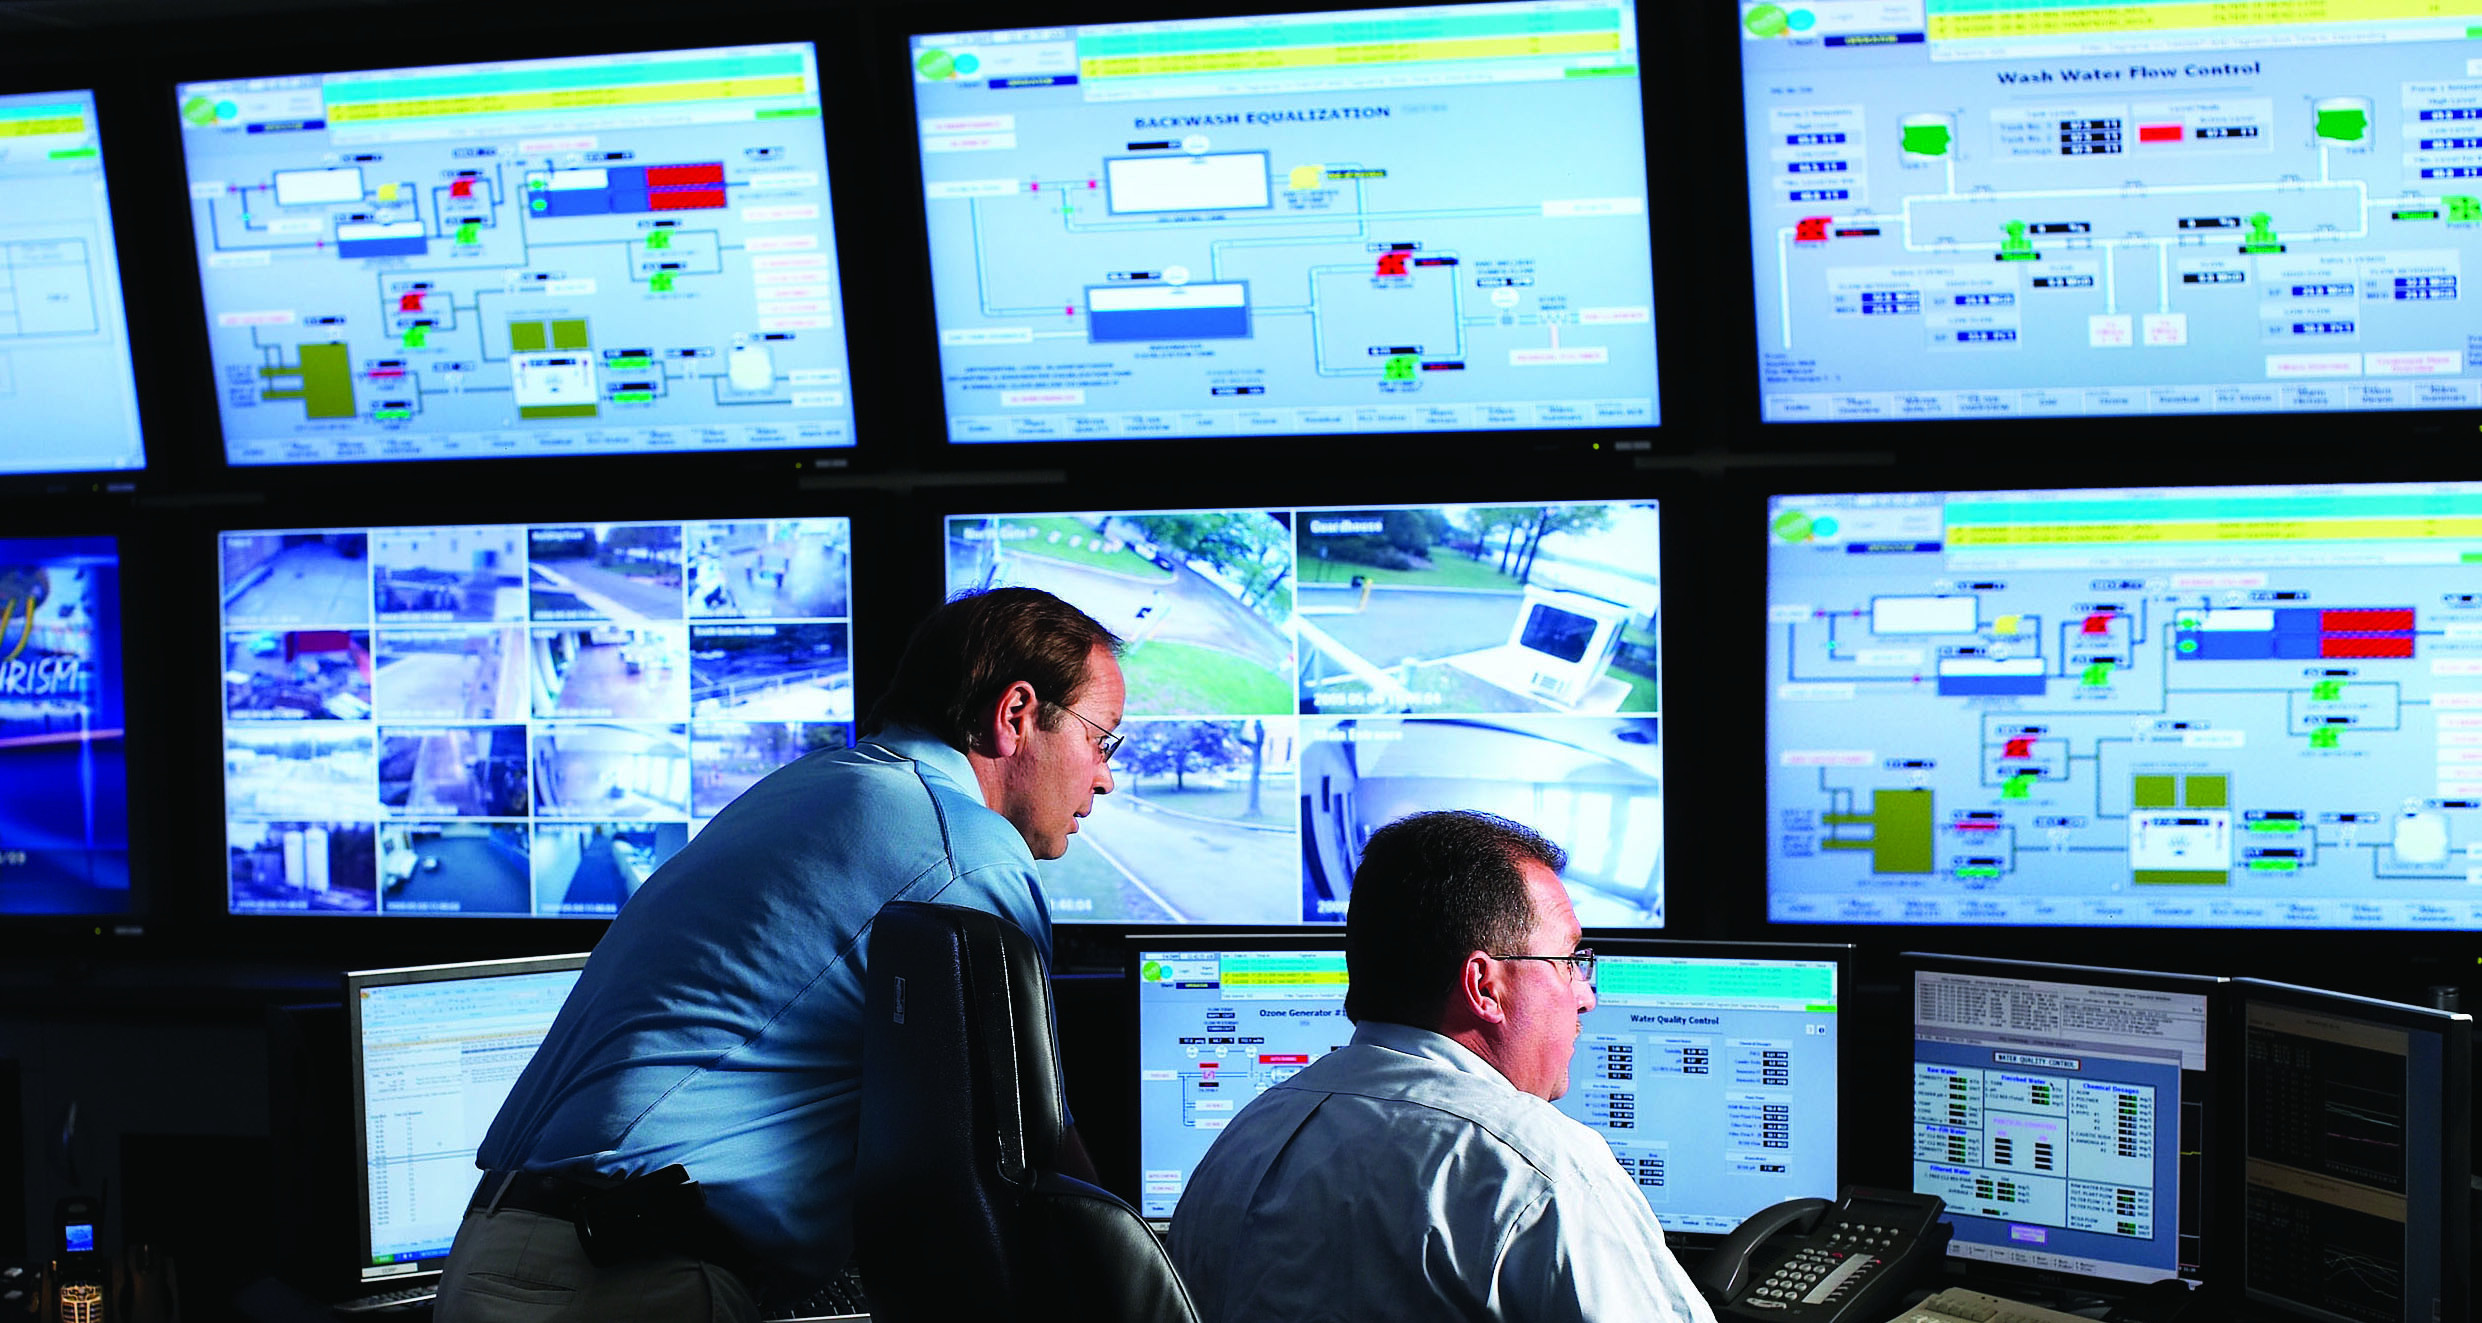
\includegraphics{scada}
                        }
                    \end{column}
                    \begin{column}{.3\textwidth}
                        \resizebox{\textwidth}{!}{
                            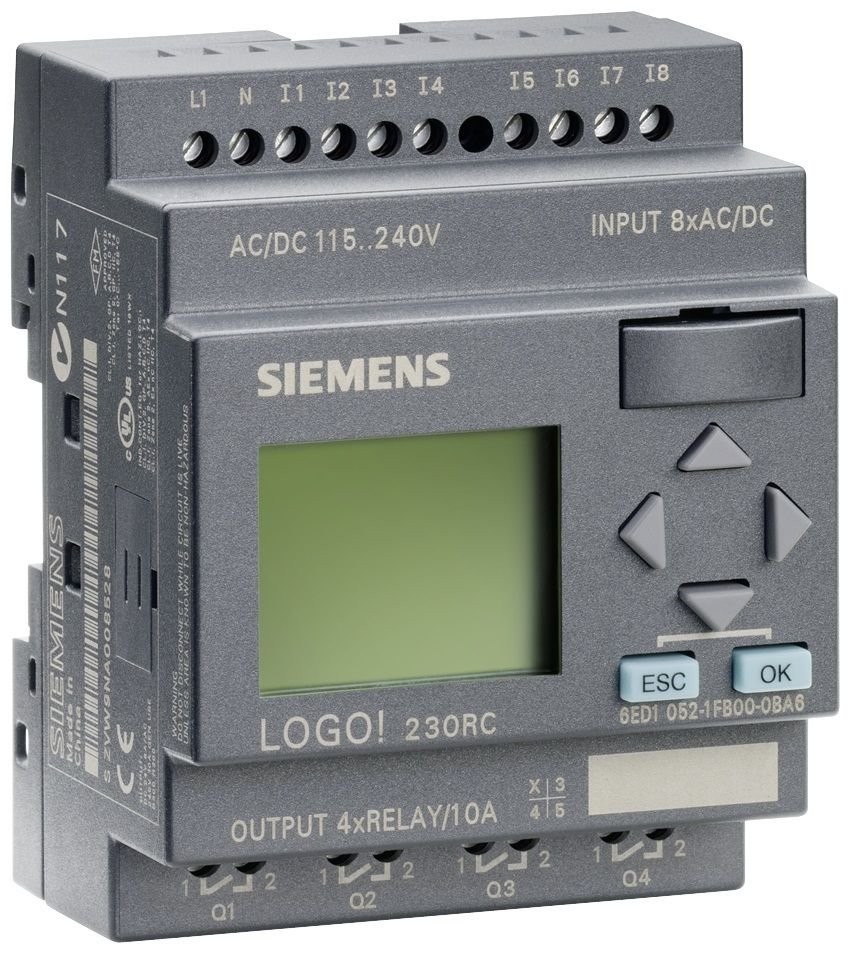
\includegraphics{plc}
                        }
                    \end{column}
                    \begin{column}{.3\textwidth}
                        \resizebox{\textwidth}{!}{
                            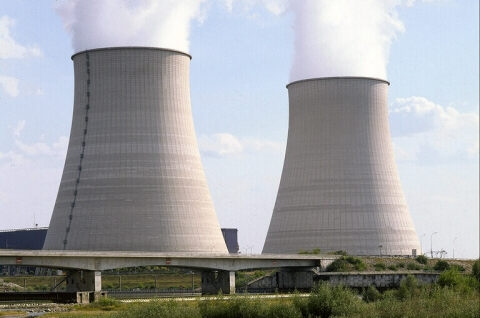
\includegraphics{plant}
                        }
                    \end{column}
                \end{columns}
                \vspace{.4em}
                \begin{itemize}
                    \item Increasing number of attacks showed in the medias since Stuxnet.
                    \item Becoming a priority for government agencies.
                    \begin{itemize}
                        \item LPM to ensure the security of OIVs.
                        \item Publications from ANSSI, DGA, ...
                    \end{itemize}
                \end{itemize}
            \end{tcolorbox}
        \end{column}
        %\hfill
        \begin{column}{.49\textwidth}
            \begin{tcolorbox}[adjusted title={\centering\large Security concepts}]
                \begin{itemize}
                    \item Safety = Protection against identified/natural difficulties.
                    \begin{itemize}
                        \item Historic industrial concern.
                    \end{itemize}
                    \item \Cybersec = Protection against malicious adversaries.
                    \begin{itemize}
                        \item Often called Security.
                    \end{itemize}
                \end{itemize}

                \begin{figure}[htb]
                    \resizebox{.85\columnwidth}{!}{
                        \def\rectangle{(-1.5,-4.5) rectangle (12,5.25)}
\def\secondcircle{(0:15.75) ellipse (6 and 4.5)}
\def\thridcircle{(0:-5.25) ellipse (6 and 4.5)}
\def\fourthcircle{(0:5.25) ellipse (6.75 and 3)}

\begin{tikzpicture}
    \draw \rectangle node at (5.25,4) {Industrial systems};
    \draw \secondcircle node {\Cybersec};
    \draw \thridcircle node {Safety};
    \draw \fourthcircle node [align=center]{Industrial \\ systems \\ \cybersec};
    \begin{scope}[fill opacity=0.25]
        \fill[blue]   \rectangle;
        \fill[red]    \secondcircle;
        \fill[green]  \thridcircle;
        \fill[yellow] \fourthcircle;
    \end{scope}
\end{tikzpicture}

                    }
                    \vspace{-.2cm}
                    \caption{Relations among security concepts}
                \end{figure}
                \vspace{-.5cm}
                \begin{itemize}
                    \item Ludovic Pietre-Cambacedes' thesis: On the relationships between safety and security, Telecom ParisTech and EDF, 2010.
                \end{itemize}
            \end{tcolorbox}
        \end{column}
    \end{columns}
    \vfill
    \begin{tcolorbox}[adjusted title={\centering\large Formal Analysis of SCADA Protocols}]
        \vspace{.5em}
        \begin{columns}[T]
            \begin{column}{.35\textwidth}
                \begin{tcolorbox}[
                colback=white, %background color of the box
                colframe=normalTitleBlockColor, %color of frame and title background
                colframe=gray!20, %color of frame and title background
                boxrule=1mm,
                coltext=black, %color of body text
                coltitle=black, %color of title text
                bottom=2mm,
                equal height group=B,
                valign = center,
                adjusted title={\large Objectives}]
                    \vspace{.5em}
                    \begin{itemize}
                        \item Modeling in the {\bf $\pi$-calculus language} of:
                        \begin{itemize}
                            \item Industrial protocols such as \modbus and \opcua.
                            \item Security properties of secrecy and authentication.
                        \end{itemize}
                    \vspace{.5em}
                        \item Analyze by the {\bf \proverif} prover:
                        \begin{itemize}
                            \item Intruder follows decisional {\bf Dolev-Yao} model.
                            \item Results: either a formal proof of security or an attack trace.
                        \end{itemize}
                    \vspace{.5em}
                        \item Literature involves analysis of e-voting, e-cash, e-reputation, e-exams, etc.
                    \vspace{.5em}
                    \item SCADA systems requires more complex properties: {\bf integrity} and {\bf availability}.
                    \end{itemize}
                \end{tcolorbox}
            \end{column}
            \begin{column}{.65\textwidth}
                \begin{tcolorbox}[
                colback=white, %background color of the box
                colframe=normalTitleBlockColor, %color of frame and title background
                colframe=gray!20, %color of frame and title background
                boxrule=1mm,
                coltext=black, %color of body text
                coltitle=black, %color of title text
                bottom=2mm,
                equal height group=B,
                valign = center,
                adjusted title={\large Approach}]
                    \begin{columns}[T]
                        \begin{column}{.45\textwidth}
\begin{lstlisting}
Cli = cCE!0xcafe -> cCE?0xcafe -> OK
E = cCE?M -> if M==0xcafe then cES!0xdead
             else cES!M -> cES?M ->
             if M==0xdead then cCE!0xcafe
             else cCE!M
Srv = c?M -> if M==0xdead then BAD -> c!M
Sys = Cli [|c|] E [|c|] Srv
assert Sys =\=> (BAD and OK)
\end{lstlisting}
                        \end{column}
                        \begin{column}{.55\textwidth}
                            \begin{figure}[htb]
                                \resizebox{\textwidth}{!}{
                                    \includegraphics{opcua}
                                }
                                \caption{\opcua OpenSecureChannel sub-protocol}
                            \end{figure}
                        \end{column}
                    \end{columns}
                \end{tcolorbox}
            \end{column}
        \end{columns}
    \end{tcolorbox}
    \vfill
    \begin{tcolorbox}[adjusted title={\centering\large Smart-Fuzzing of SCADA Systems}]
        \vspace{.5em}
        \begin{columns}[T]
            \begin{column}{.35\textwidth}
                \begin{tcolorbox}[
                colback=white, %background color of the box
                colframe=normalTitleBlockColor, %color of frame and title background
                colframe=gray!20, %color of frame and title background
                boxrule=1mm,
                coltext=black, %color of body text
                coltitle=black, %color of title text
                bottom=2mm,
                equal height group=C,
                valign = center,
                adjusted title={\large Objectives}]
                    \vspace{.5em}
                    \begin{itemize}
                        \item Modeling in the {\bf CSP language} of:
                        \begin{itemize}
                            \item SCADA infrastructures (components, network links and communication protocols),
                            \item Threats (in terms of position, capacities and objectives),
                            \item Security objectives (\eg "This services needs authentication.") and safety properties (\eg "Electricity consumption always remains lower than production").
                        \end{itemize}
                        \item Automaticaly produce abstract attack scenarios that an adversary should follow to achieve one of his objective using the {\bf FDR3 model-checker}.
                        \item Convert attack scenarios to real network packets with the {\bf Scapy} python package to verify and quantify their plausibility.
                    \end{itemize}
                \end{tcolorbox}
            \end{column}
            \begin{column}{.65\textwidth}
                \begin{tcolorbox}[
                colback=white, %background color of the box
                colframe=normalTitleBlockColor, %color of frame and title background
                colframe=gray!20, %color of frame and title background
                boxrule=1mm,
                coltext=black, %color of body text
                coltitle=black, %color of title text
                bottom=2mm,
                equal height group=C,
                valign = center,
                adjusted title={\large Approach}]
                    \begin{columns}[T]
                        \begin{column}{.5\textwidth}
                            \begin{figure}[htb]
                                \vspace{1.5em}
                                \resizebox{.95\columnwidth}{!}{
                                    \begin{tikzpicture}[
        arrow/.style={thick,->,shorten >=2pt,shorten <=2pt,>=stealth},
    ]
    \draw (2,6) rectangle (5,7) node [pos=.5] {Architecture};
    \draw (6,6) rectangle (9,7) node [pos=.5] {Prop. de sécurité};


    \draw (4,4) rectangle (7,5) node [pos=.5] {Analyses};

    \draw (0,2) rectangle (3,3) node [pos=.5] {Bibliothèque};
    \draw (4,0) rectangle (7,1) node [pos=.5] {Paquets};
    \draw (8,2) rectangle (11,3) node [pos=.5] {Contexte};

    \draw (4,2) rectangle (7,3) node [align=center,pos=.5] {Instanciation\\Concrétisation};

    \draw[arrow] (3.5,6) -- (5.5,5); % Archi --> Analyses
    \draw[arrow] (7.5,6) -- (5.5,5); % Props --> Analyses
    \draw[arrow] (5.5,4) -- (5.5,3) node [pos=.5,right] {Suite d'actions décrivant des attaques}; % Analyses --> Inst
    \draw[arrow] (3,2.5) -- (4,2.5); % Biblio --> Inst
    \draw[arrow] (8,2.5) -- (7,2.5); % Context--> Inst
    \draw[arrow] (5.5,2) -- (5.5,1); % Inst --> Packets
\end{tikzpicture}

                                }
                                \vspace{-.25em}
                                \caption{Our global approach}
                            \end{figure}
                        \end{column}
                        \begin{column}{.5\textwidth}
                            \vspace{.5em}
                            \begin{figure}[htb]
\begin{lstlisting}
Cli = cCE!0xcafe -> cCE?0xcafe -> OK
E = cCE?M -> if M==0xcafe then cES!0xdead
             else cES!M -> cES?M ->
             if M==0xdead then cCE!0xcafe
             else cCE!M
Srv = c?M -> if M==0xdead then BAD -> c!M
Sys = Cli [|c|] E [|c|] Srv
assert Sys =\=> (BAD and OK)
\end{lstlisting}
                                \caption{Modeling example (CSP-like)}
                            \end{figure}
                            \vspace{.5em}
                            \begin{figure}[htb]
                                \resizebox{.95\columnwidth}{!}{
                                    \begin{tikzpicture}[font=\Large,
    arrow/.style={thick,->,shorten >=2pt,shorten <=2pt,>=stealth},
]
    \draw (0,0) rectangle (2,1) node [pos=.5] {$Client$};
    \draw[fill=red!20!white] (5,0) rectangle (7,1) node [pos=.5] {$Enemy$};
    \draw (10,0) rectangle (12,1) node [pos=.5] {$Server$};

    % Clients - Servers links
    \draw[arrow] (2,.75) -- (5,.75)  node [anchor=south, pos=.5, align=center, above=.5em] {Write(0xbeef, 0xcafe)};
    \draw[arrow] (7,.75) -- (10,.75) node [anchor=south, pos=.5, align=center, above=.5em] {Write(0xbeef, {\color{red!75!black} 0xdead})};
    \draw[arrow] (10,.25) -- (7,.25)   node [anchor=north, pos=.5, align=center, below=.5em] {Write(0xbeef, 0xdead)};
    \draw[arrow] (5,.25) -- (2,.25)    node [anchor=north, pos=.5, align=center, below=.5em] {Write(0xbeef, {\color{red!75!black} 0xcafe})};
\end{tikzpicture}

                                }
                                \vspace{-.5em}
                                \caption{Attack example}
                            \end{figure}
                        \end{column}
                    \end{columns}
                \end{tcolorbox}
            \end{column}
        \end{columns}
        \begin{tcolorbox}[
        colback=white, %background color of the box
        colframe=normalTitleBlockColor, %color of frame and title background
        colframe=gray!20, %color of frame and title background
        boxrule=1mm,
        coltext=black, %color of body text
        coltitle=black, %color of title text
        bottom=2mm,
        equal height group=C,
        valign = center,
        adjusted title={\large Attack Models}]
        \end{tcolorbox}
    \end{tcolorbox}
    \vfill
\end{frame}

\end{document}

